\documentclass{beamer}
\usepackage[utf8]{inputenc}
\usepackage[T1]{fontenc}
\usepackage{graphicx}
\usepackage{tcolorbox}
\usepackage{hyperref}
\hypersetup{
    colorlinks=true,
    linkcolor=pink,
    urlcolor=cyan,
    urlbordercolor=cyan,
}
\graphicspath{ {./images/} }

\usetheme{Arguelles}

\title{Tutorial 3}
\subtitle{CS3241 Computer Graphics (AY23/24)}
\date{\today}
\author{Wong Pei Xian}
\institute[]{\email{e0389023@u.nus.edu}}

\begin{document}

\frame[plain]{\titlepage}

\section{Question 1}

\begin{frame}
    \frametitle{Question 1a}

    \begin{tcolorbox}[colback=teal!5!white]
        \textcolor{teal}{pollev.com/peixian}
    \end{tcolorbox}

    Given three points A, B, and C in 3D space, write an expression for the \textbf{normal vector}
    of the plane that contains the three points.
\end{frame}

\begin{frame}
    \frametitle{Normal vector}

    \begin{center}
        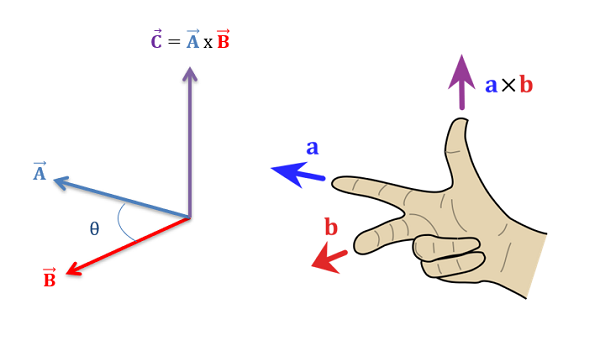
\includegraphics[scale=0.6]{images/cross-prod-righthand.png}
    \end{center}

    \begin{align*}
        \mathbf{a} &:= B - A \\
        \mathbf{b} &:= C - A \\
        \mathbf{n} &:= \mathbf{a} \times \mathbf{b} \\
        &= (B-A) \times (C-A)
    \end{align*}


\end{frame}

\begin{frame}
    \frametitle{Question 1b}

    Given a point $R = [r_x \  r_y \  r_z]^T$ on a plane $\Pi$ and a normal vector 
    $n = [n_x \  n_y \  n_z]^T$ of the plane, write the implicit-form equation of 
    the plane in the form $ax + by + cz + d = 0$.

\end{frame}

\begin{frame}
    \frametitle{Implicit form}

    \begin{center}
        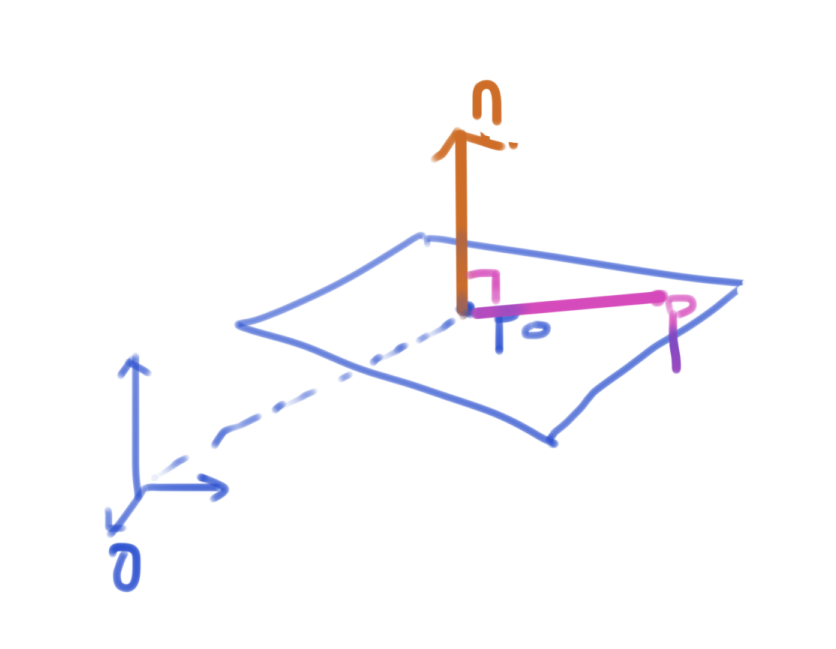
\includegraphics[scale=0.4]{plane-def.png}

        \begin{eqnarray}
            n \cdot ([x \  y \  z]^T - R) &= 0 \\ 
            n_x x + n_y y + n_z z - n\cdot R &= 0
        \end{eqnarray}
    \end{center}

\end{frame}

\begin{frame}
    \frametitle{Question 1c}
    
    What is the perpendicular distance of the point $Q$ from the plane $ax + by + cz + d = 0$?

\end{frame}

\begin{frame}
    \frametitle{Perpendicular distance of point to plane}

    Let $Q = [q_x \  q_y \  q_z]^T$. Then the distance $D$ from point to plane is 

    \begin{eqnarray}
        D = \left| \frac{aq_x + bq_y + cq_z + d}{\sqrt{a^2 + b^2 + c^2}}\right|
    \end{eqnarray}

\end{frame}

\begin{frame}
    \frametitle{Proof?}

    \begin{center}
        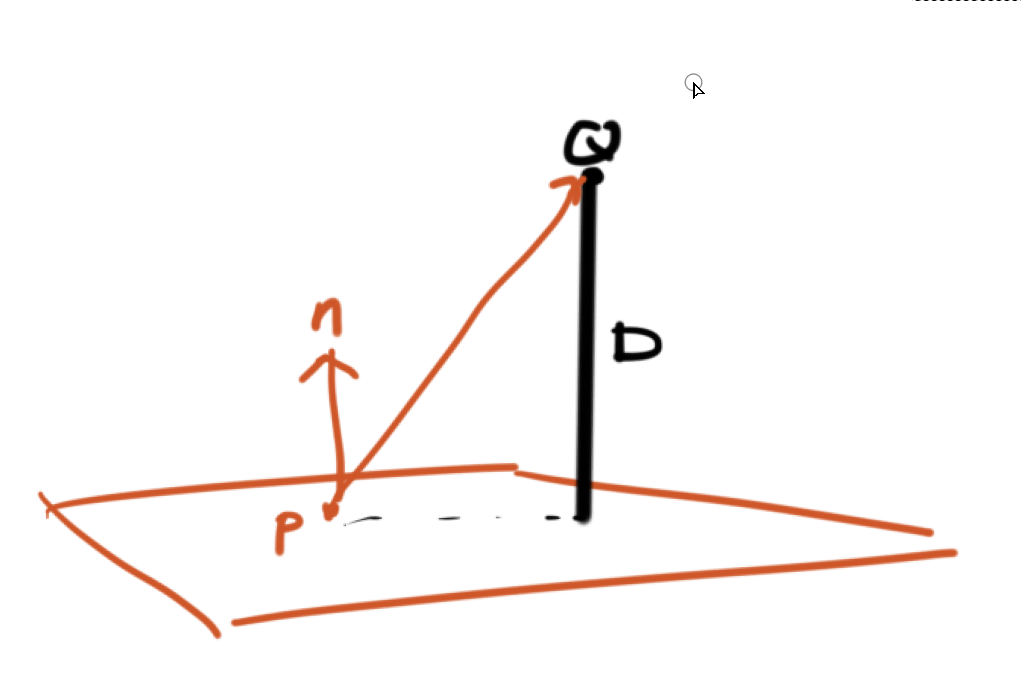
\includegraphics[scale=0.5]{distance_perp.png}
    \end{center}

\end{frame}

\begin{frame}
    \frametitle{Outline of proof}

    \begin{eqnarray*}
        D &= \|PQ\| \cos \theta \\
        &= \|PQ\| \text{norm}(n) \cdot \text{norm}(PQ) \\
        &= \|PQ\| \frac{n \cdot PQ}{\|n\| \|PQ\|} \\
        &= \frac{n \cdot (OQ - OP)}{\|n\|} \\ 
        &= \frac{\textcolor{teal}{n \cdot OQ} - \textcolor{blue}{n \cdot OP}}{\textcolor{red}{\|n\|}} \\
        &= \frac{\textcolor{teal}{n_x x + n_y y + n_z z} - (\textcolor{blue}{-d})}{\textcolor{red}{\sqrt{a^2 + b^2 + c^2}}}\\
    \end{eqnarray*}

\end{frame}

\section{Question 2}

\begin{frame}
    \frametitle{Question 2a}

    \begin{tcolorbox}[colback=teal!5!white]
        \textcolor{teal}{pollev.com/peixian}
    \end{tcolorbox}

    \vspace{1em}
    
    What does the homogenous coordinates $[6, 4, 2, 0.5]^T$ represent?

\end{frame}

\begin{frame}
    \frametitle{Question 2a}

    What does the homogenous coordinates $[6, 4, 2, 0.5]^T$ represent?

    \begin{tcolorbox}
        \begin{eqnarray*}
            & \left[
            \begin{matrix}
                x & y & z & w
            \end{matrix} 
            \right]\\
            = & \left[
            \begin{matrix}
                x/w & y/w & z/w & 1
            \end{matrix}
            \right]
        \end{eqnarray*}
    \end{tcolorbox}
    

\end{frame}

\begin{frame}
    \frametitle{Question 2b}

    Why does OpenGL (and many other graphics APIs) use homogeneous coordinates to represent points?

\end{frame}

\begin{frame}
    \frametitle{Why homogenous coordinates?}

    \begin{enumerate}
        \item Different representations for points and vectors.
        \item $4 \times 4$ Matrix multiplication
        \item Perspective projection with matrix mult. and \textit{perspective division}.
    \end{enumerate}
    
\end{frame}

\begin{frame}
    \frametitle{Point vector distinguishing}

    For \textbf{vector}; $w = 0$ \quad e.g. $\left[ \begin{matrix}
        x & y & z & 0
    \end{matrix} \right]$.

    For \textbf{point}; $w = 1$ \quad e.g. $\left[ \begin{matrix}
        x & y & z & 1
    \end{matrix} \right]$.

    \begin{tcolorbox}
        In this week's lecture, you will learn that to transform \textbf{normal vectors} instead of points,
        we use the matrix
        \begin{eqnarray*}
            M_n = (M_t^{-1})^T
        \end{eqnarray*}
        where $M_t$ is the upper left $3 \times 3$ submatrix.
    \end{tcolorbox}

\end{frame}

\section{Question 3}

\begin{frame}
    \frametitle{Question 3}

    \begin{tcolorbox}[colback=teal!5!white]
        \textcolor{teal}{pollev.com/peixian}
    \end{tcolorbox}

    Which of the followings is the matrix that rotates objects about the fixed 3D point 
    $[2 \  3 \  4]^T$, where the rotation axis is parallel to and in the same direction 
    as the x-axis, and the rotation angle is $\theta$? 

    \begin{center}
        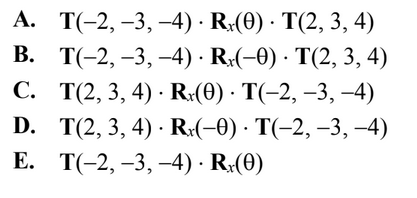
\includegraphics[scale=0.8]{q3-options.png}
    \end{center}

\end{frame}

\begin{frame}
    \frametitle{Things to note about transformation}


    \begin{center}
        
\includegraphics[scale=0.4]{order-of-trans.png}
    \end{center}

\end{frame}

\begin{frame}
    \frametitle{Things to note about transformation}


    \begin{center}
        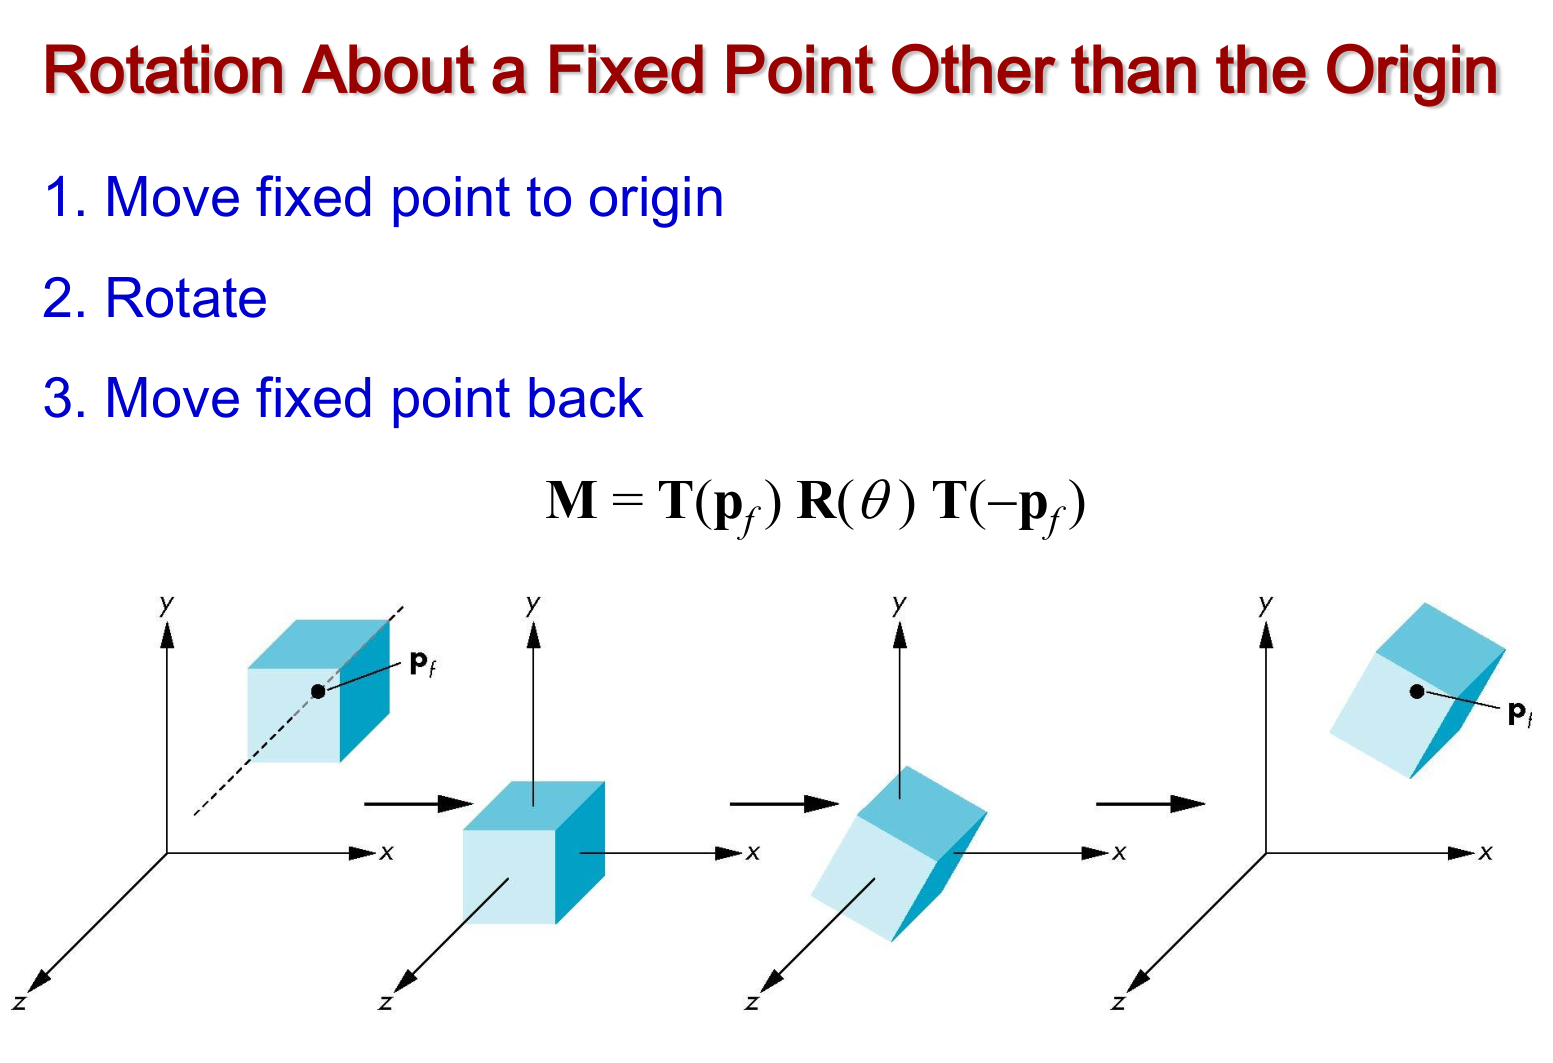
\includegraphics[scale=0.3]{rotate-about-fixed-pt.png}
    \end{center}

    \begin{tcolorbox}
        Ans: $T(2,3,4) \cdot R(\theta) \cdot T(-2, -3, -4)$.
    \end{tcolorbox}

\end{frame}

\section{Question 4}

\begin{frame}
    \frametitle{Question 4}

    What is the inverse matrix of 

    \begin{center}
        $$ M = 
        \left[
        \begin{matrix}
            s_1 r_{11} & s_1 r_{12} & s_1 r_{13} & t_1\\
            s_2 r_{21} & s_2 r_{22} & s_2 r_{23} & t_2\\
            s_3 r_{31} & s_3 r_{32} & s_3 r_{33} & t_3\\
            0 & 0 & 0 & 1
        \end{matrix}
        \right]
        $$
        
    \end{center}

\end{frame}

\begin{frame}
    \frametitle{Step 1: Decompose}

    You can tell there is a $S$, $R$, and $T$ matrix multiplied together in some order to give $M$.

    $$ R = 
    \left[
    \begin{matrix}
        r_{11} & r_{12} & r_{13} & 0\\
        r_{21} & r_{22} & r_{23} & 0\\
        r_{31} & r_{32} & r_{33} & 0\\
        0 & 0 & 0 & 1
    \end{matrix}
    \right],
    S =
    \left[
    \begin{matrix}
        s_{11} & 0 & 0 & 0\\
        0 & s_{22} & 0 & 0\\
        0 & 0 & s_{33} & 0\\
        0 & 0 & 0 & 1
    \end{matrix}
    \right],
    T =
    \left[
    \begin{matrix}
        1 & 0 & 0 & t_1\\
        0 & 1 & 0 & t_2\\
        0 & 0 & 1 & t_3\\
        0 & 0 & 0 & 1
    \end{matrix}
    \right]
    $$

\end{frame}

\begin{frame}
    \frametitle{Step 2: Order}

    \begin{tcolorbox}[colback=teal!5!white]
        \textcolor{teal}{pollev.com/peixian}
    \end{tcolorbox}
    
    $M =$ ?

\end{frame}

\begin{frame}
    \frametitle{Step 2: Order}

    $M = TSR$.

    \vspace{1em}

    Thus $M^{-1} = R^{-1} S^{-1} T^{-1}$.

\end{frame}

\begin{frame}
    \frametitle{How to get here}

    \begin{enumerate}
        \item Trial and error
        \item Hints
        \begin{itemize}
            \item In $M$, the last column $[\begin{matrix}t_1 & t_2 & t_3 & 1\end{matrix}]^T$ is not transformed.
            \item i.e. $T$ applied \textbf{last}
            \item $M = TRS$ or $M = TSR$
        \end{itemize}
    \end{enumerate}

\end{frame}

\begin{frame}
    \frametitle{Step 3: Substitute and Compute}

    \begin{center}
        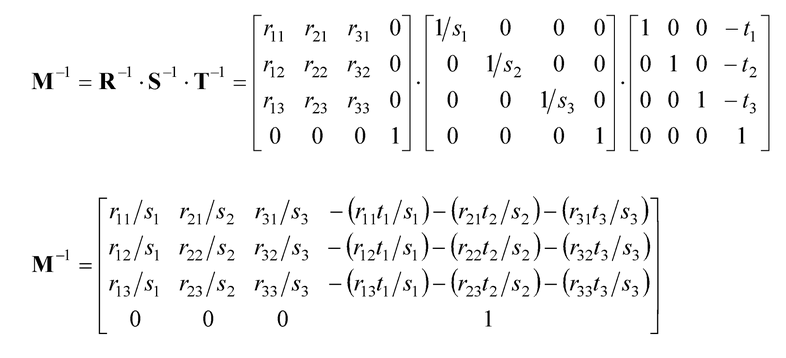
\includegraphics[scale=0.6]{q4.png}
    \end{center}

\end{frame}

\section{Question 5}

\begin{frame}
    \frametitle{Question 5}
    
    Let $M_1 = TR$. \\
    Let $M_2 = RT$. \\
    Is $M_1 = M_2$? Prove it.

\end{frame}

\begin{frame}
    \frametitle{Experiment with hand}

    \begin{enumerate}
        \item With left hand, define 3 axes. This is \textbf{object space}. 
        \item Your left hand is now at \textbf{world space} origin
        \begin{enumerate}
            \item \textcolor{blue}{Translate your hand by $T = [0, 0, 5]$.}
            \item \textcolor{teal}{Rotate your hand by $R_x(90^o)$.}
            \item Note where is your hand now in \textbf{world space}.
        \end{enumerate}
        \item Now reset your left hand to the \textbf{world space} origin
        \begin{enumerate}
            \item \textcolor{teal}{Rotate your hand by $R_x(90^o)$.}
            \item \textcolor{blue}{Translate your hand by $T = [0, 0, 5]$.}
        \end{enumerate}
        \item \textit{Is your hand in the space world space position as before?}
    \end{enumerate}

\end{frame}

\begin{frame}
    \frametitle{Proof and counterexample}

    \begin{tcolorbox}
        In general $TR \neq RT$.
    \end{tcolorbox}

    i.e. $M_1 \neq M_2$. Counterexample:

    $$T(1, 0, 0) R_z(\pi/2) P(1, 0, 0) \neq R_z(\pi/2) T(1, 0, 0) P(1, 0, 0)$$
    $$P(1, 1, 0) \neq P(0, 2, 0)$$

    (Note: $P(x,y,z)$ refers to the point $(x,y,z)$.)

\end{frame}

\section{Question 6}

\begin{frame}
    \frametitle{Question 6}

    The computation of $\sin \theta$ and $\cos \theta$ is considered relatively slow 
    for some real-time rendering applications. \\

    \vspace{1em}

    However, when the angle $\theta$ is very small, we can make use of the small-angle 
    approximation: $\sin \theta \approx \theta$, and $\cos \theta \approx 1 - \theta_{small}/2$, 
    for better speed.\\

    \vspace{1em}
    
    Write the 4x4 matrix for rotation about the z-axis by a very small rotation angle $\theta_{small}$, 
    which is given in radians. 

\end{frame}

\begin{frame}
    \frametitle{Substitute in}

    \begin{center}
        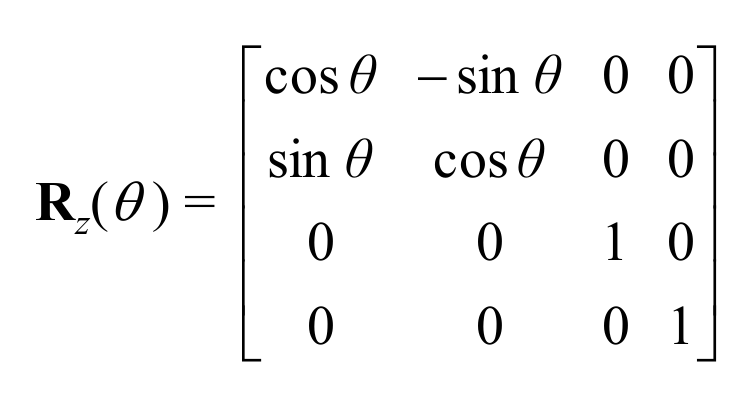
\includegraphics[scale=0.3]{rot-mat.png}
    \end{center}
    
    \begin{tcolorbox}
        $$ \cos \theta \approx 1 - \theta^2_{small}/2 $$
        $$ \sin \theta \approx \theta_{small} $$
    \end{tcolorbox}

\end{frame}

\begin{frame}
    \frametitle{Substitute in}

    \begin{align*}
    \mathbf{R}_Z(\theta) &= \left[ \begin{matrix}
        \cos\theta & -\sin\theta & 0 & 0 \\
        \sin\theta & \cos\theta & 0 & 0 \\
        0 & 0 & 1 & 0 \\
        0 & 0 & 0 & 1 \\
    \end{matrix} \right] \\
    &\approx \left[ \begin{matrix}
        1 - \theta_{small}^2/2 & -\theta_{small} & 0 & 0 \\
        \theta_{small} & 1 - \theta_{small}^2/2 & 0 & 0 \\
        0 & 0 & 1 & 0 \\
        0 & 0 & 0 & 1 \\
    \end{matrix} \right]
    \end{align*}

\end{frame}

\section{Question 7}

\begin{frame}
    \frametitle{Question 7}

    In OpenGL, what is the purpose of transforming vertices to window space?

\end{frame}

\begin{frame}
    \frametitle{For the rasterizer!}

    \begin{center}
        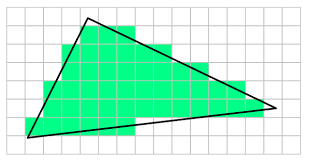
\includegraphics[scale=0.6]{rasterizer.png}
    \end{center}

\end{frame}

\section{Question 8}

\begin{frame}
    \frametitle{Question 8}

    \begin{tcolorbox}[colback=teal!5!white]
        \textcolor{teal}{pollev.com/peixian}
    \end{tcolorbox}

    What are the matrices applied to each vertex $v_1 \dots v_6$?

\end{frame}

\begin{frame}
    \frametitle{Question 8}

    \begin{center}
        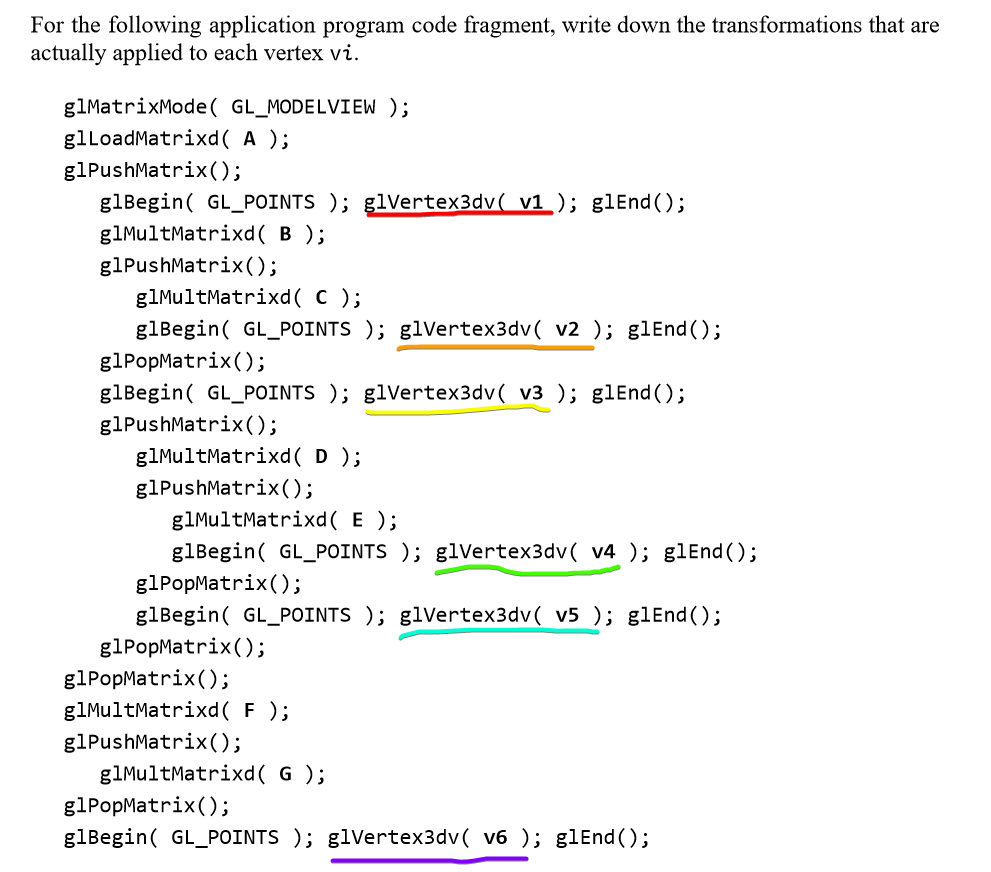
\includegraphics[scale=0.5]{q8.png}
    \end{center}

\end{frame}

\begin{frame}
    \frametitle{OpenGL's matrix stacks API}

    \label{matrixAPI}

    \begin{itemize}
        \item \texttt{glMatrixMode}: sets matrix being modified to either ModelView or Projection.
        \item \texttt{glLoadMatrix/glLoadIdentity}: clears entire matrix stack and replaces with loaded matrix/identity matrix $I$
        \item \texttt{glMultMatrix}: \textbf{postmultiplies} matrix to the current stack
        \begin{itemize}
            \item Note that the stack grows from left to right as a result.
        \end{itemize}
        \item \texttt{glPushMatrix}: creates a new "sub-stack" of matrices (see next slides for actual implementation)
        \item \texttt{glPopMatrix}: pops-off the previous "sub-stack" of matrices
    \end{itemize}

\end{frame}

\begin{frame}
    \frametitle{Understanding OpenGL's matrix stacks}

    \begin{center}
        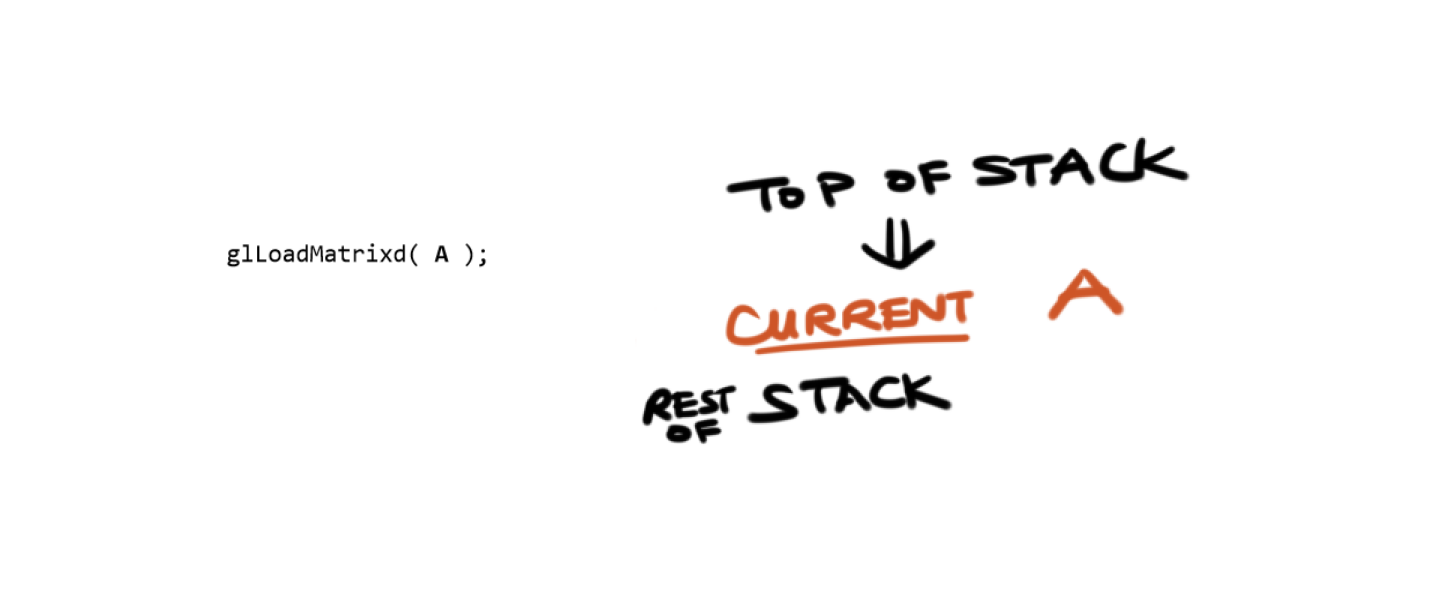
\includegraphics[scale=0.4]{q8-1.png}
    \end{center}

    \small
    In fact, OpenGL works with a stack of stack of matrices.
    For clarity, the outer stack will be referred to as the stack, 
    and the matrices being multiplied together will be referred to as the product.

    On \texttt{glLoadMatrix}, the stack is initialized with one product (the single matrix $A$ in this example).

\end{frame}

\begin{frame}
    \frametitle{Understanding OpenGL's matrix stacks}

    \begin{center}
        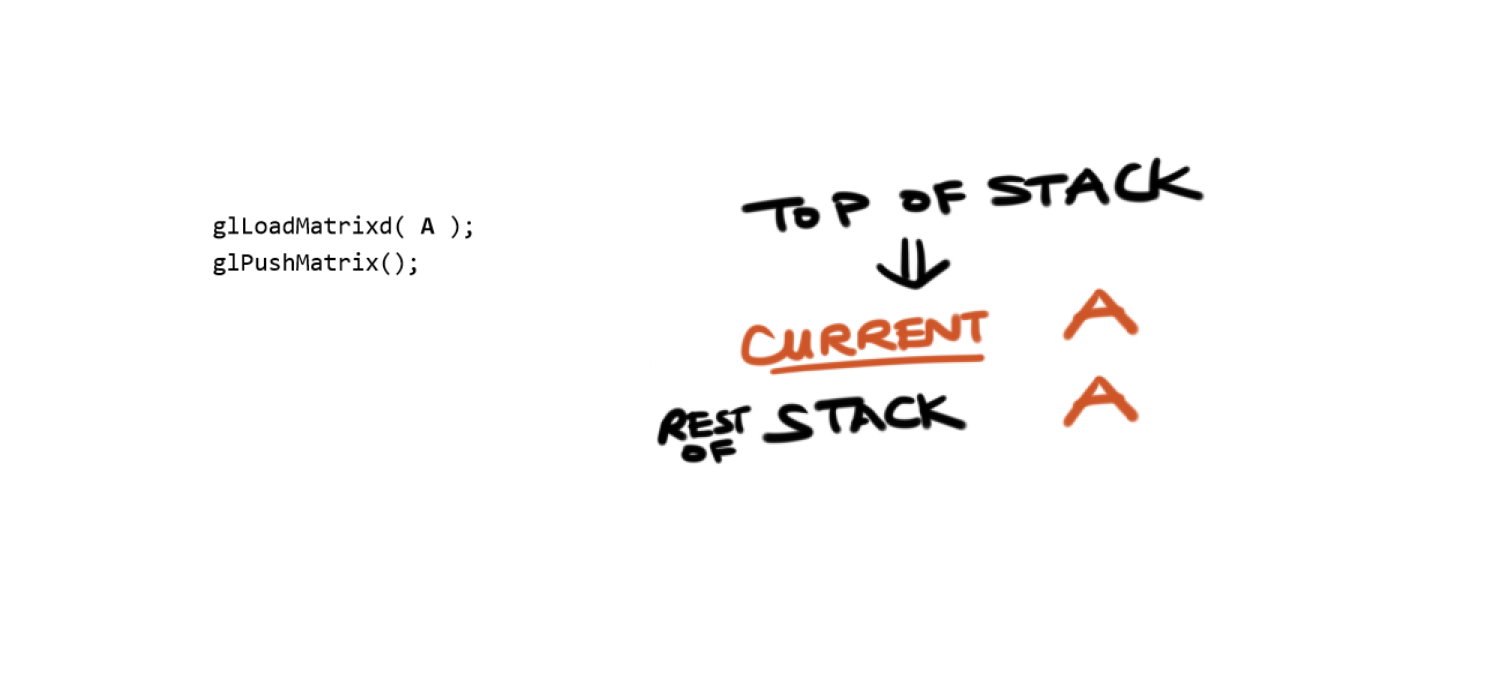
\includegraphics[scale=0.4]{q8-2.png}
    \end{center}

    When \texttt{glPushMatrix} is called, the top product of the stack is 
    duplicated and added to the top of the stack.

\end{frame}

\begin{frame}
    \frametitle{Understanding OpenGL's matrix stacks}

    \begin{center}
        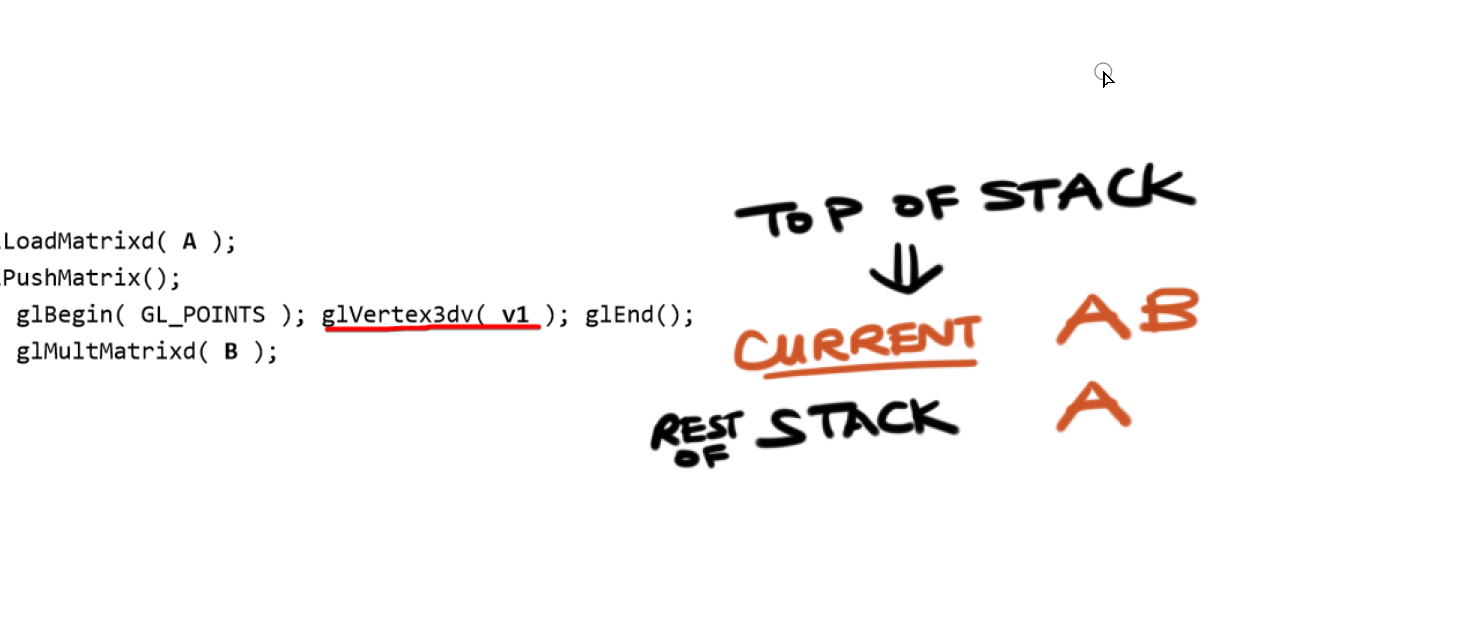
\includegraphics[scale=0.4]{q8-3.png}
    \end{center}

    When \texttt{glMultMatrix} is called, the matrix $B$ is post-multiplied to the current
    product at the top of the stack $A$.

\end{frame}

\begin{frame}
    \frametitle{Understanding OpenGL's matrix stacks}

    \begin{center}
        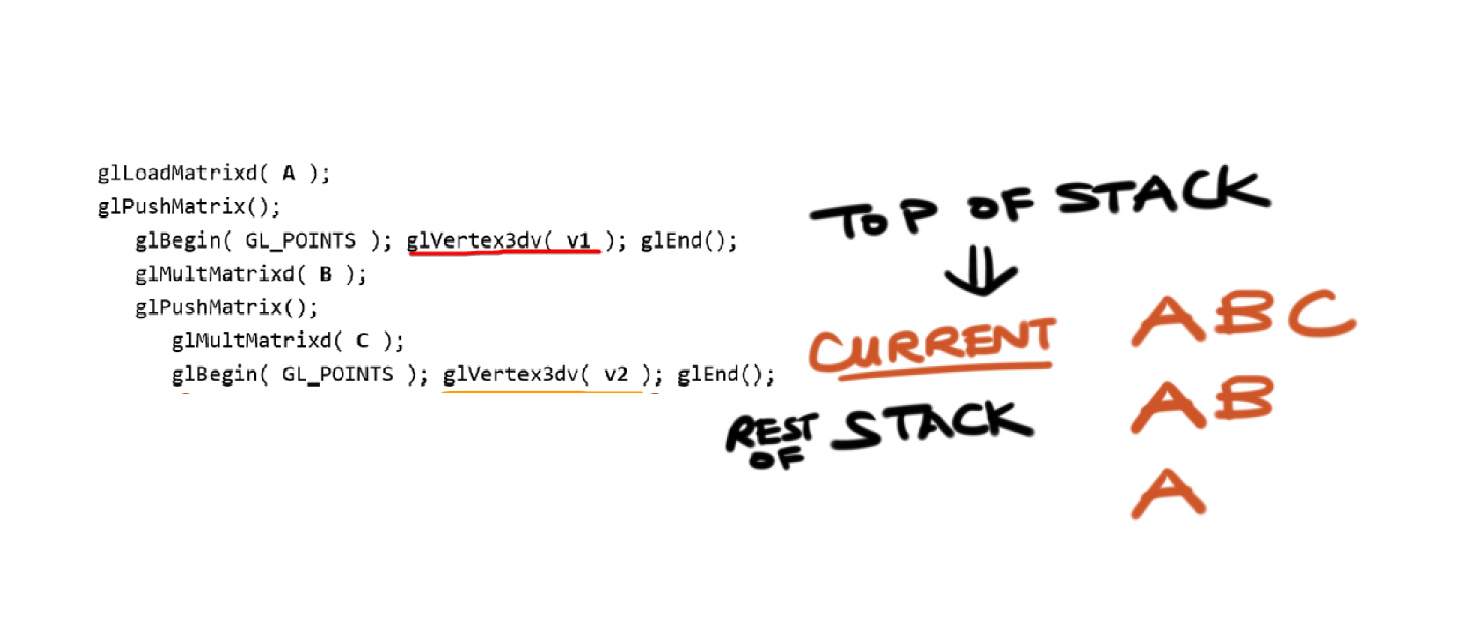
\includegraphics[scale=0.4]{q8-4.png}
    \end{center}

    This is similarly applied here.

\end{frame}

\begin{frame}
    \frametitle{Understanding OpenGL's matrix stacks}

    \begin{center}
        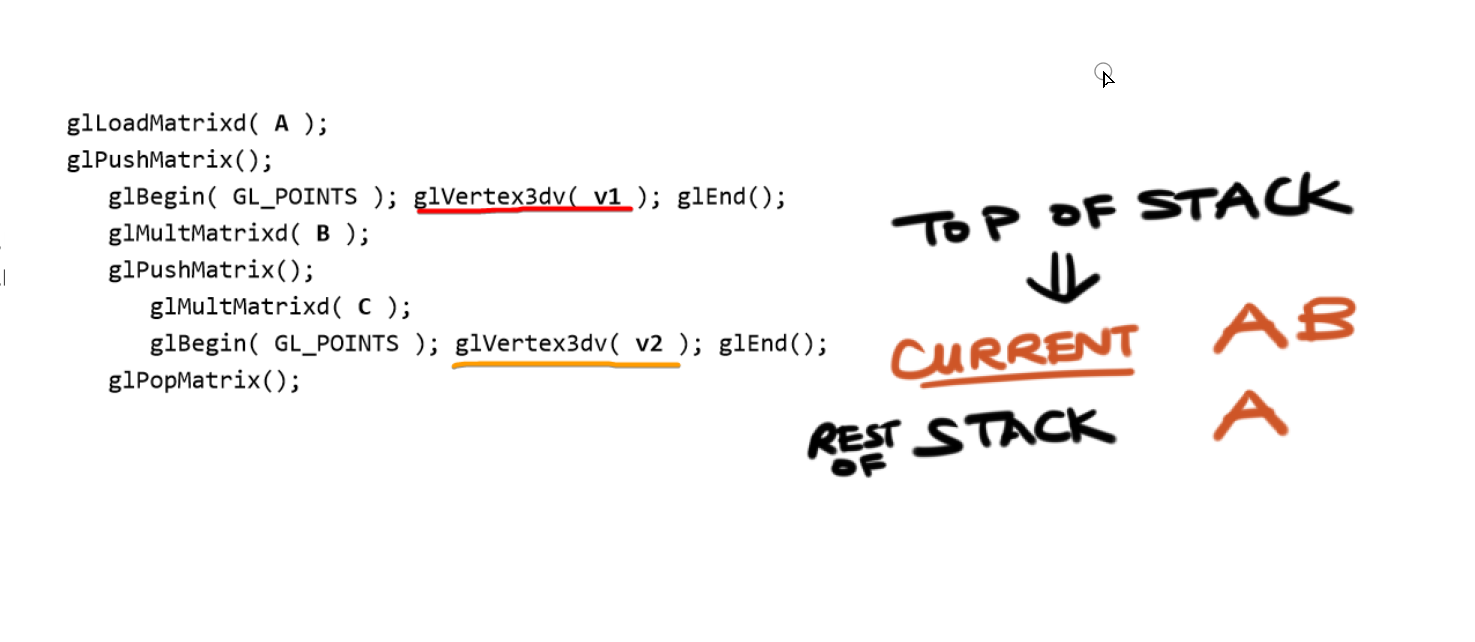
\includegraphics[scale=0.4]{q8-5.png}
    \end{center}

    When \texttt{glPopMatrix} is called, the top-most product in the stack
    is removed.

\end{frame}

\begin{frame}
    \frametitle{Note that}

    \begin{enumerate}
        \item \texttt{glMultMatrix} \textbf{post-multiplies} the current matrix
        \item \texttt{glPushMatrix} makes a copy of the topmost matrix of the stack, and makes it the current matrix
        \item \texttt{glPopMatrix} deletes the top-most matrix and replaces it with the next one on the stack.
        \item \texttt{glLoadIdentity} replaces the \textbf{current matrix} with $I$.
    \end{enumerate}

    If too confusing, the high level understanding from here (slide \ref{matrixAPI}) suffices.

\end{frame}

\begin{frame}[plain,standout]
    \AlegreyaExtraBold \LARGE
    Attendance taking
\end{frame}

\ThankYou
\begin{frame}[plain,standout]
    Thanks! Get the slides here after the tutorial.\\
    \vspace{2em}
    \scalebox{3}{\faGithub}\par\bigskip
    \url{https://trxe.github.io/cs3241-notes}\\
    \vspace{3em}
    {\small Feel free to ask me questions about Assignment 1.  }
\end{frame}

\end{document}